\documentclass[12pt]{article}

\usepackage{titling}
\usepackage{setspace}
\usepackage{fancyhdr}
\usepackage{indentfirst}
\usepackage{graphicx}
\usepackage{amsmath}
\usepackage{amssymb}

\graphicspath{{./images/}}

% Tech Note Space and a Half Format
\begin{document}

% Header
% ----------------------------------
\onehalfspacing
\thispagestyle{fancy}
\fancyhf{}
\lhead{\textbf{Revision Number: 002} \\ \textbf{Date: \today} \\ \textbf{From: Ryan Bugianesi} \\ \textbf{Subject: LSTM Neural Network Notes}}
\setlength{\headheight}{56.18335pt}

\section{Introduction}

This document details the design of a Long-Short Term Memory (LSTM) neural
network. The design and structure for this network was inspired from videos by
Josh Starmer [1] and Ahlad Kunar [2] on YouTube. All diagrams shown in this
document are credited to Josh Starmer and are included for visualization.

% Video Link: https://www.youtube.com/watch?v=YCzL96nL7j0
% Video Link: https://www.youtube.com/watch?v=8rQPJnyGLlY&t=1789s

\section{Implementation}

The LSTM network is implemented in C++ using an object-oriented approach from a
`bottom up' perspective. The gates within the architecture were designed first
and incorporated into more abstract classes.

\subsection{Classes}

\subsubsection{ForgetGate}

The ForgetGate class implements the first stage of a LSTM network neuron. This
class uses the long-term memory, short-term memory, and input values to
determine how much of the long-term memory is propagated to the rest of the
architecture. The ForgetGate class accomplishes this by using a sigmoid
activation function. After scaling the inputs by the saved biases and weights
specific to this class only, the sum of the weighted input, the weighted value
of the short-term memory, and the bias are used as the input to a sigmoid
function. The result of this calculation represents the percentage of the
long-term memory to keep. The long-term memory is then updated via
multiplication with the output of the sigmoid function. A value of 1 would
represent the propagation of the long term memory value, while 0 would cause
the information to be lost, or ``forgotten'' to the network.

Figure 1, shown below, gives a visualization of the first stage. The green line
represents the long term memory propagating through the entire neuron.
Similarly, the red line represents the short-term memory. The input to the
neuron is shown in the blue box, and its path is shown by the gray line.

\begin{center}
    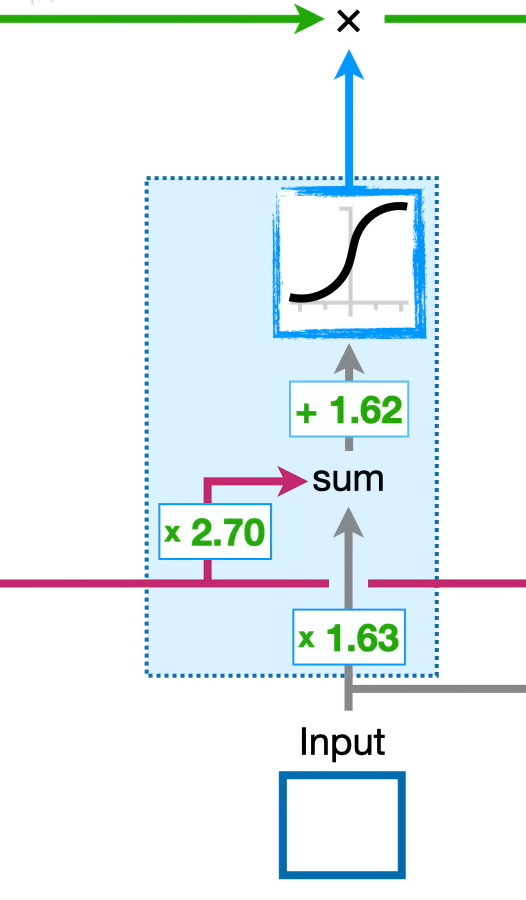
\includegraphics[width=0.5\textwidth]{ForgetGate.png}\\
    \emph{Figure 1 - LSTM Forget Gate}
\end{center}
To understand how the data propagates through the network more clearly, it
helps to express the operations through math. This also helps later when
calculating error. To begin, the input gate's operation can be expressed as:
\begin{equation}
    \label{eqn:f_t}
    f_t = \sigma(x_t*U_f + h_{t-1}*W_f + b_f)
\end{equation}

Where $x_t$ is the input to the gate at time \emph{t}, $h_{t-1}$ is the value
of the hidden state, or short-term memory, at time $t - 1$, and $U_f$, $W_f$,
and $b_f$ are the weights and biases of the Forget Gate.

This equation will be used later when training the network for comparing error
between expected value and predicted value ($f_t$).

\subsubsection{InputGate}

The Input Gate class implements the second function of a LSTM neuron. This
class manages updating the long term memory with new information. Again, all
three internal values are used to create the new memory. The green line (long
term memory) gets an additional value added to it (representing the new
information). This additional value is computed by the two blocks shown in
Figure 2. The green block represents the calculation the network uses to
determine how much of the new information is to be saved. Using the sum of the
input value (gray line) and the short term memory value (red line), multiplied
by their corresponding weights, the LSTM network calculates the value of the
sigmoid function. This calculation returns a value between 0 and 1. This value
is the percent of the new long term memory to be added to the existing long
term memory.

The orange block uses the same values as the green block, with different
weights, to calculate the actual value of the new long term memory. The block
has a special name: the \textbf{candidate state}, and is discussed in The
Architecture section. This calculation uses the $\tanh$ function. This function
returns a value between -1 and 1, which represents the new information.

After completing the calculations of both blocks, the product of the computed
values is added to the long term memory.

\begin{center}
    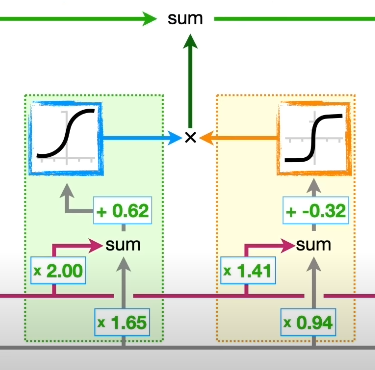
\includegraphics{InputGate.png}\\
    \emph{Figure 2 - LSTM Input Gate}
\end{center}

The Input Gate's operation can be described by:

\begin{equation}
    \label{eqn:i_t}
    i_t = \sigma(x_t*U_i + h_{t-1}*W_i + b_i)
\end{equation}

Where $x_t$ is the input to the gate at time \emph{t}, $h_{t-1}$ is the value
of the hidden state, or short-term memory, at time $t - 1$, and $U_i$, $W_i$,
and $b_i$ are the weights and biases of the Input Gate.

\subsubsection{Output Gate}

The output gate (shown in \emph{Figure 3} below) is in charge of generating the
next short term memory to be passed on as output from an arbitrary neuron. This
process is done in the same manner as the long term memory generation in the
Input Gate. The inputs to this block of the LSTM neuron are the short term
memory value, the input value, and the long term memory value.

The short term memory is used along with the input value and corresponding
weights to generate a sum. This sum is added to a bias value and passed to a
sigmoid function to normalize the value to the range of 0-1. The output value
from the sigmoid function determines how much of the new short term memory is
saved.

The long term memory is used to determine the value of the new short term
memory. By passing the value of the long term memory generated in the previous
stage to a $\tanh()$ function. The output value of this function is combined
with the output of the sigmoid function in the adjacent block. This output
value is the new short term memory, and it is an output of neuron.

\begin{center}
    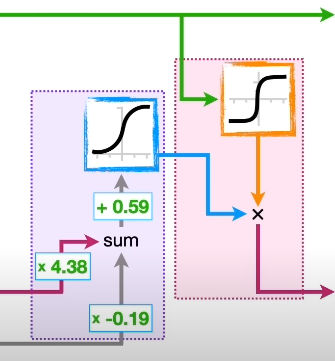
\includegraphics{OutputGate.png}\\
    \emph{Figure 3 - LSTM Output}
\end{center}

The Output Gate's operation can be described by:

\begin{equation}
    \label{eqn:o_t}
    o_t = \sigma(x_t*U_o + h_{t-1}*W_o + b_o)
\end{equation}

Where $x_t$ is the input to the gate at time \emph{t}, $h_{t-1}$ is the value
of the hidden state, or short-term memory, at time $t - 1$, and $U_o$, $W_o$,
and $b_o$ are the weights and biases of the Output Gate.

\section{Architecture}

The data is propagated through the network of gates by calculating the outputs
of each gate and performing operations on the internal short and long term
``memory'' (a.k.a. the hidden state and cell state respectively). The
operations performed on these internal values can be represented by the
following equations:

\begin{equation}
    C_t = f_t*C_{t-1} + i_t*g_t
\end{equation}
\begin{equation}
    H_t = o_t*\tanh(C_t)
\end{equation}

Where $C_t$ and $H_t$ are the new values of the short and long term memory
(Cell and Hidden states) at time $t$ and $g_t$ is the value of the candidate
state:

\begin{equation}
    \label{eqn:g_t}
    g_t = \tanh(x_t*U_g + h_{t-1}*W_o + b_g)
\end{equation}

The output of the network at a time $t$ can be checked by performing the
calculation for $H_t$ and is often filtered through a `softmax' function to
normalize the output to a probability distribution when the network is built
using multidimensional data (i.e. $x_t \in \mathbb{R}^n$ where $n > 1$).

The overall architecture can be represented succinctly by Equation 5. When
performing back propagation, the derivative of this equation is needed. The
chain rule can be used to calculate the derivatives of Equations 1-4 to be used
in the calculation of Equation 5.

\subsection{Backwards Propagation  (Training)}

Given some input $x$, the LSTM network predicts some output value, $y$. By
comparing the predicted value of $y$ to the actual known value of $y$, the
parameters of the network can be tuned to increase its performance, resulting
in a smaller difference between $y_{expected}$ and $y_{predicted}$. This
process is called backwards propagation and is a common technique used to train
predictive models.

The following algorithm is used to determine how to update the tunable weights
and biases of the network for a given input value and known expected value:

\begin{equation}
    W_{new} = W_{old} - (\frac{dL}{dW} * \alpha)
\end{equation}

Where $W_{new}$ represents the updated parameter, $W_{old}$ represents the
original value of the parameter, $\frac{dL}{dW}$ represents the derivative of
the \textbf{Loss Function} with respect to the parameter, and $\alpha$
represents a value called the \textbf{Learning Rate}. The loss function and
learning rate are discussed in later sections.

In a LSTM architecture, loss is computed for each LSTM unit in time. For
instance,

\begin{equation}
    L = \sum_{t=0}^{T}L_t
\end{equation}

Where each $L_t$ with $0 \le t \le T$ represents the loss of the LSTM network
at a given time. In other words, the loss, or error, of the network at a given
time $t$ is the summation of the loss (error) of each intermediate calculation
between 0 and $T$.

The loss function to be evaluated first is the Residual Sum of Squares (RSS)
loss function.

\begin{equation}
    L_t = (y_i - H(x_i))^2
\end{equation}

Where $y_i$ is the i$^{th}$ value to be predicted, $H_i(x_i)$ is the prediction
from the model with input $x_i$ Backwards propagation is performed by
calculating the derivative of $L$ with respect to each of the weights and
biases. That is, we need to calculate:

\begin{equation*}
    \frac{\partial L}{\partial U_i}, \frac{\partial L}{\partial U_f}. \frac{\partial L}{\partial U_o}, \frac{\partial L}{\partial U_g}, \frac{\partial L}{\partial W_i}, \frac{\partial L}{\partial W_f}, \frac{\partial L}{\partial W_o}, \frac{\partial L}{\partial W_g}
\end{equation*}

To calculate all these values, keep in mind that the derivatives of the $\tanh$
and $\sigma$ functions are known:

\begin{equation}
    \sigma'(x) = \sigma(x)(1-\sigma(x))
\end{equation}
\begin{equation}
    \tanh'(x) = 1 - (\tanh(x))^2
\end{equation}

In general, to calculate the derivatives of the loss function with respect to
each of the tunable parameters, follow the chain rule for taking partial
derivatives. That is, $\frac{\partial L}{\partial param} = (\frac{\partial L}{\partial gate}) (\frac{\partial gate}{\partial param})$.

For this network, the loss function used is the RSS loss function, so:

\begin{subequations}
    \begin{align}
        L_t & = (y_t - H_t(x_t))^2                                 \\
        L_t & = (y_t - (o_t\tanh((C_t))))                          \\
        L_t & = (y_t - (o_t \tanh((f_t)(C_{t-1}) + (i_t)(g_t))))^2
    \end{align}
\end{subequations}

Recall equations \ref{eqn:f_t}, \ref{eqn:i_t}, \ref{eqn:o_t} and \ref{eqn:g_t}
which describe $f_t$, $i_t$, $o_t$ and $g_t$. Already the complexity of
equation 12c is almost intolerable. This is why the chain rule is useful.

First,

\begin{math}
    a
\end{math}

\subsubsection{Loss Function}

The loss function is simply a way to represent the calculated error of the
model. There are many useful loss functions that are applicable to different
scenarios and machine learning models. For example, Mean Squared Error (MSE),
Mean Absolute Error (MAE) and Mean Bias Error (MBE) to name a few.

It is best practice to use cross-validation to determine the best loss function
for a set of particular data. For this reason, this document will assume the
use of a basic loss function to simplify the calculations shown. It is a good
idea to implement many options after gaining a basic understanding of the
algorithms and architecture.

\subsubsection{Learning Rate}

The learning rate is a small number that is used to scale the value that
updates the parameters of the model being trained. This value is important
because it changes the resolution of the training. If this value was omitted
and the derivative of the loss function yielded a large value, the training
algorithm could skip over an optimal value of the parameter being updated.
Including this value reduces the likelihood of this scenario.

\section{Conclusion}
The LSTM neural network aims to fix the problem of vanishing gradients present
in basic and recurrent neural networks by only allowing incremental updates to
the recurrent state.

\end{document}